\appendix
\section{Appendix}
\subsection{Code for Penultimate Layer Representation} \label{sec:app_pen}
\begin{algorithm}[ht]
\vspace{0.2em}\scriptsize
\begin{minted}[xleftmargin=2em, numbersep=6pt, linenos, breaklines]{python}
import numpy as np

# normalize a vector
def normalize(v):
    norm = np.linalg.norm(v)
    return v / norm


def qr_decomposition(points):
    # construct the matrix A from the templates
    A = np.zeros((2, points.shape[1]))
    A[0] = normalize(points[1] - points[0])
    A[1] = normalize(points[2] - points[0])

    # apply the QR decomposition
    Q, R = np.linalg.qr(A.T)

    # return the orthogonal matrix (orthonormal basis)
    return Q


# get w_1, w_2, and w_3
templates = penultimate_weights[class_indices]
# construct the matrix and apply the QR decomposition
orthonormal_basis = qr_decomposition(templates)

# project the penultimate layer activations on the plane for each class
for i in range(3):
    projection[i] = np.dot(penultimate_activations[i], orthonormal_basis)
\end{minted}
\vspace{-0.5em}
\caption{Code for calculating the penultimate layer representation}
\end{algorithm}
\subsection{Overview Over Experiments}
\begin{table}[ht]
    \centering
    \footnotesize
    \caption{Overview of all model and dataset combinations and the experiments where these combinations were used. The used abbreviations are: Accuracy (Accuracy with label smoothing, see Section \ref{sec:acc}), PLR (Penultimate layer representation, see Section \ref{sec:plr}), IMC (Implicit model calibration, see Section \ref{sec:imc}), and KD (Knowledge distillation, see Section \ref{sec:kd})}
    \renewcommand{\arraystretch}{1.4}
    \begin{tabular}{|c|c|P{4em}P{4em}P{4em}P{4em}|}
    \hline
    %\Xhline{3\arrayrulewidth}\\[-3.0em]
         & & \multicolumn{4}{c|}{\sc Experiment}\\
         %\cline{3-6}
         \sc Dataset & \sc Architecture & Accuracy & PLR & IMC & KD\\
         %\Xhline{2\arrayrulewidth}
         \hline
         \sc \hyperref[mnist]{MNIST} & \sc \hyperref[fc_model]{FC} & \checkmark & \checkmark & \checkmark & \checkmark\\
         \hline
         \sc \hyperref[emnist]{EMNIST} & \sc \hyperref[fc_model]{FC} & \checkmark & & \checkmark & \\
         \hline
         \sc \hyperref[fmnist]{FMNIST} & \sc \hyperref[fc_model]{FC} & \checkmark & & \checkmark & \\
         \hline
         \sc \hyperref[cifar10]{CIFAR-10} & \sc \hyperref[alexnet_model]{AlexNet} & \checkmark & \checkmark & \checkmark & \checkmark\\
         \hline
         \sc \hyperref[cifar10]{CIFAR-10} & \sc \hyperref[resnet56_model]{ResNet56} & \checkmark & & \checkmark & \checkmark\\
         \hline
         \sc \hyperref[cifar100]{CIFAR-100} & \sc \hyperref[resnet56_model]{ResNet-56} & \checkmark & \checkmark & \checkmark & \\
         \hline
         \sc \hyperref[cub200]{CUB-200-2011} & \sc \hyperref[resnet34_model]{ResNet-34} & \checkmark & \checkmark & \checkmark & \\
         \hline
         \sc \hyperref[imagenet]{Tiny ImageNet} & \sc \hyperref[resnet50_model]{ResNet-50} & \checkmark & \checkmark & \checkmark & \\
         \hline
         \sc \hyperref[multi30k]{Multi30k} & \sc \hyperref[transformer_model]{Transformer} & & & \checkmark & \\
         \hline
         %\Xhline{3\arrayrulewidth}
    \end{tabular}
    
    \label{tab:overview}
\end{table}
\clearpage
\subsection{Further Reliability Diagrams}

\begin{figure}[ht]
\centering
    \begin{subfigure}{.45\textwidth}
    \centering
    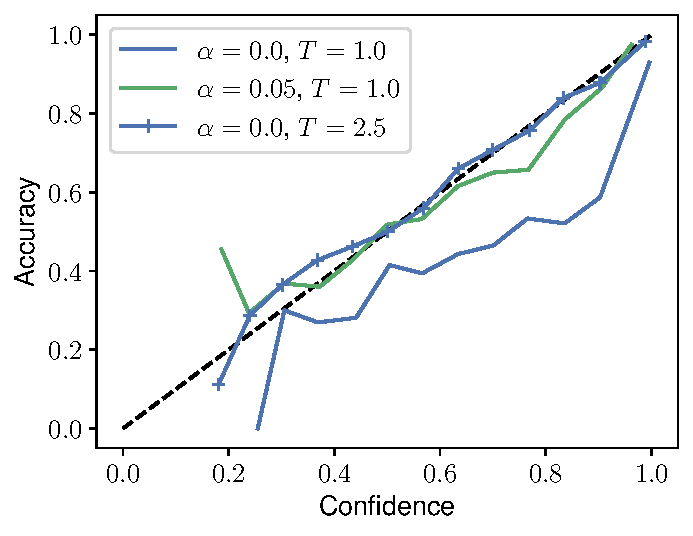
\includegraphics[width=\linewidth]{figures/reliability_alexnet_cifar10.pdf}
    \caption{AlexNet on the CIFAR-10 dataset}
\end{subfigure}
\hfill
\begin{subfigure}{.45\textwidth}
    \centering
    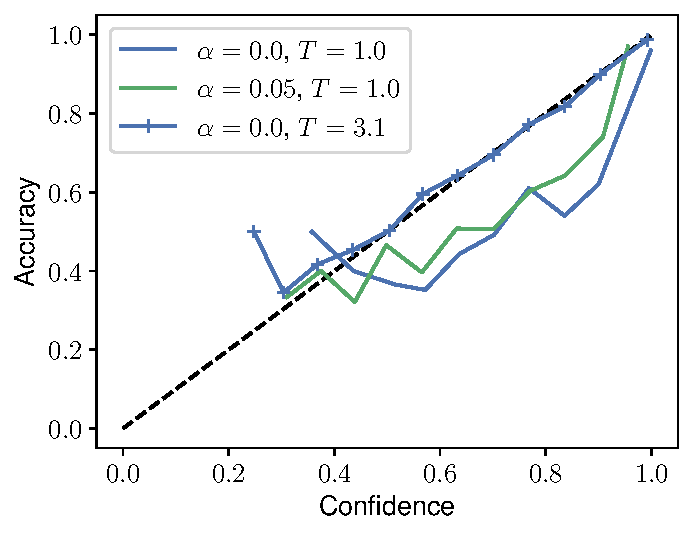
\includegraphics[width=\linewidth]{figures/reliability_resnet_cifar10.pdf}
    \caption{ResNet-56 on the CIFAR-10 dataset}
\end{subfigure}
\begin{subfigure}{.45\textwidth}
    \centering
    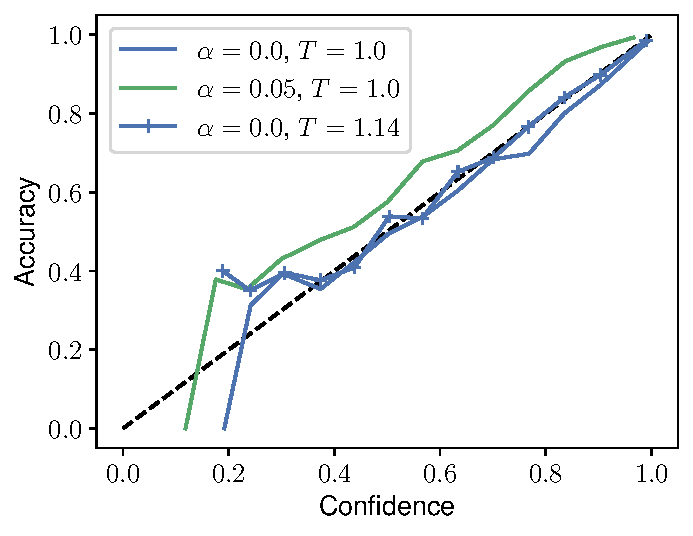
\includegraphics[width=\linewidth]{figures/reliability_emnist.pdf}
    \caption{FCN on the EMNIST dataset}
\end{subfigure}
\hfill
\begin{subfigure}{.45\textwidth}
    \centering
    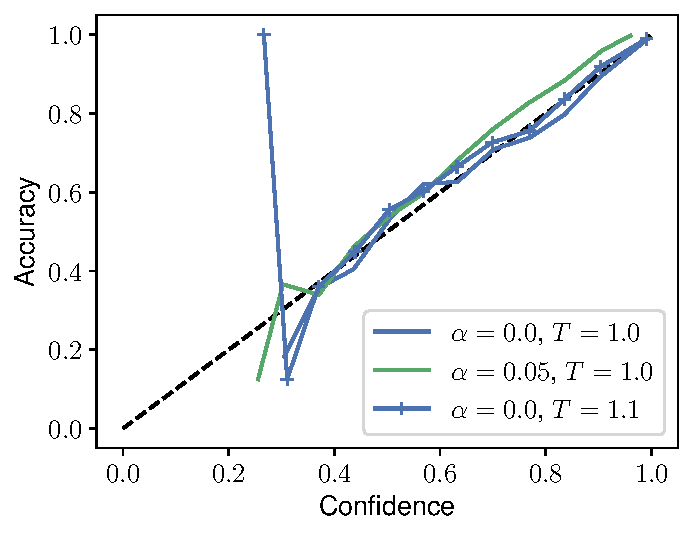
\includegraphics[width=\linewidth]{figures/reliability_fmnist.pdf}
    \caption{FCN on the FMNIST dataset}
\end{subfigure}
\begin{subfigure}{.45\textwidth}
    \centering
    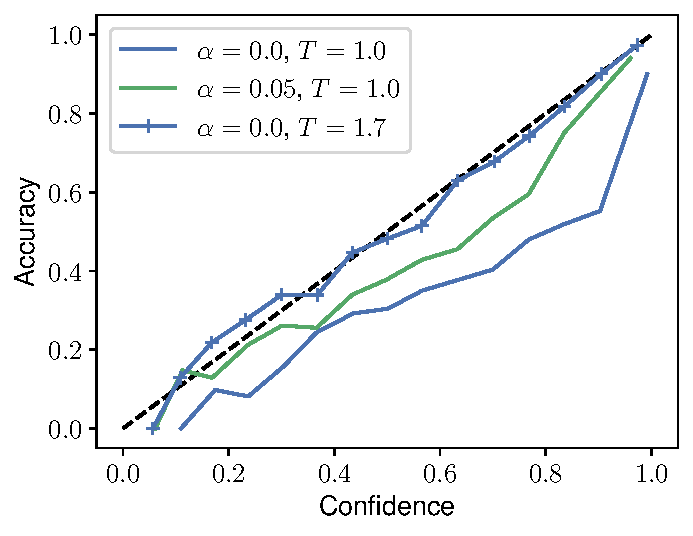
\includegraphics[width=\linewidth]{figures/reliability_resnet50_tinyimagenet.pdf}
    \caption{ResNet-50 on the Tiny ImageNet dataset}
\end{subfigure}
\hfill
\begin{subfigure}{.45\textwidth}
    \centering
    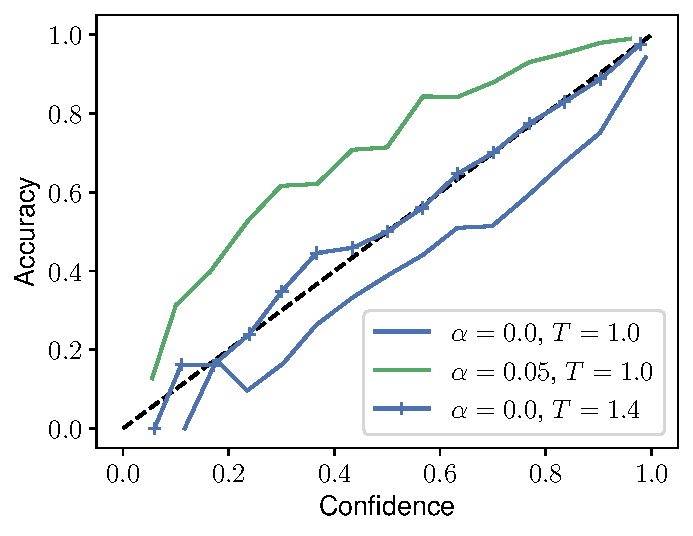
\includegraphics[width=\linewidth]{figures/reliability_resnet34_cub200.pdf}
    \caption{ResNet-34 on the CUB-200-2011 dataset}
\end{subfigure}
\caption{Reliability diagrams for various classification networks.}
\end{figure}